\documentclass{article}
\usepackage[utf8]{inputenc}
\usepackage{graphicx}
\usepackage[paper=a4paper,left=3cm, right=3cm, top=2cm]{geometry}
\usepackage{blindtext}
\usepackage{multicol}
\usepackage{pgfplots}
\usepackage{float}
\usepackage{biblatex} %Imports biblatex package
\usepackage{amsmath}
\addbibresource{main.bib} %Import the bibliography file
\usepackage{array}
\usepackage{caption}
\usepackage{subcaption}

 
\pgfplotsset{compat = newest}

\title{\textbf{Inorganic scintillator based optic fiber dosimeter}}
\author{Neelkant Newra\\
\textit{Department of Biomedical Engineering} \\ National Institute of Technology, Raipur \\ Email: newra008@gmail.com\\}
\date{}

\begin{document}
\maketitle
\begin{abstract}\textbf{This study discuss the ongoing development in the field of inorganic scintillator based optic fiber dosimeters(IOSFDs) for medical radiotherapy dosimetry, mainly targeting real-time in vivo dosimetry. SFDs (scintillator-based optical fibre dosimeters) are small, electromagnetic interference-free, radiation-resistant, and durable. They've demonstrated a lot of promise for real-time in vivo radiotherapy dosimetry.Inorganic scintillators have a greater X-ray absorption and light output than organic scintillators. The stem effect may be easily removed with variable Inorganic scintillators  that have highest emission peaks in the red region of the spectrum. In this study we will look at various advantages and disadvantages of using inorganic scintillators for SFDs fabrication. We will be also discussing about various combination of IOSDFs used for different cases. } \\ \\
    \textbf{\textit{Keywords- Inorganic scintillators, dosimetry, optical fiber}} 
\end{abstract}

\begin{multicols}{2}

\section{Introduction}

Most modern medical diagnostic imaging methods that use x-rays or gamma rays use inorganic scintillators. The relatively high detection effectiveness of inorganic scintillators for harsh radiation explains this. However, the various diagnostic procedures differ significantly, and as a result, the radiation detector needs change as well. The scintillator specs do not always meet these requirements.\cite{van2002inorganic} One of the motivations for continuing scintillator Research and Development is to address this issue. The necessity for innovative, digital diagnostic systems with good image quality and a rapid picture acquisition time, as well as excellent quality real-time imaging systems for interventional radiology with minimal radiation dosage, are the other reasons. Traditional radiotherapy approaches have well-established safety and quality guidelines, however these protocols are being challenged by the aforementioned rapidly emerging radiotherapy technologies.\cite{cowen2008design} Patients obtaining erroneous dosages while having radiation therapy using these novel radiotherapy procedures have been reported. This has raised worries about the time it takes for dosimetric equipment to catch up to treatment approaches. As a result, creating radiation dosimeters capable of real-time in vivo dose monitoring has gotten a lot of interest in the research community. Before looking at the development in the area of IOSFDs, lets use have some basic understanding of SFDs, there fundamentals, development, working , advantages and disadvantages.

\section{Fundamentals}
The fragment of scintillation material is coupled to an optical fibre in the standard SFDs arrangement. Figure 1 shows a simplified diagram of how SFDs operates in the presence of ionising radiation. When irradiated with a high-energy ionising beam, the scintillator undergoes a radioluminescence process. An optical cable collects the light photons created in the scintillator and transmits them to the photon detector (e.g., photomultiplier, CCD camera, and spectrometer). A remote computer terminal can be used to analyse the output. Theoretically The emission of scintillation light is proportional to the dosage rate in theory.\cite{stajanca2019pof} 

\begin{figure}[H]
    \centering
    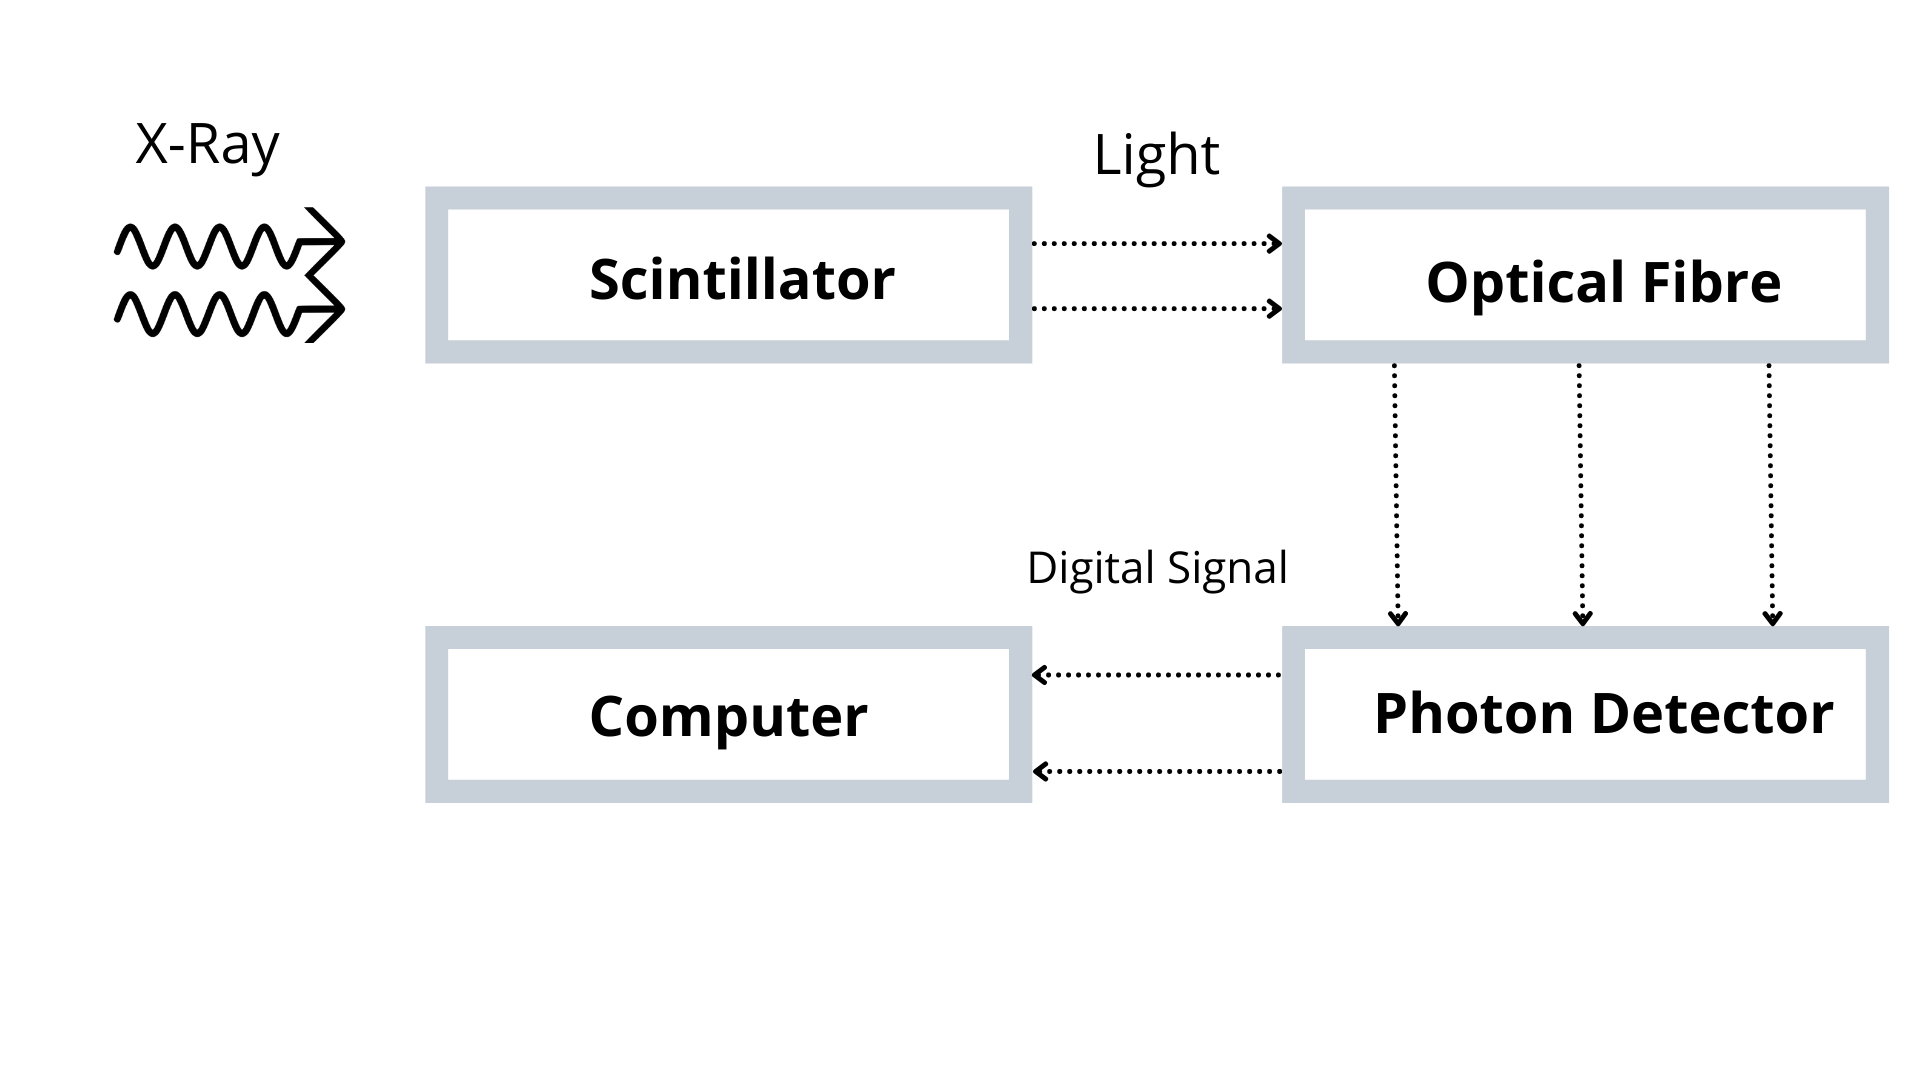
\includegraphics[width=6cm]{images/Fig1_Schematic.png}
    \caption{A simple schematic of the radiation detection process using SFDs}
    \label{fig:1}
\end{figure}

Overall, the scintillation light collecting efficiency and the scintillator's reaction to the incoming radiation particles determine the SFDs performance for oncology radiation measurement. The light collecting efficiency of scintillation is similar to the light extraction efficiency of LEDs(Light Emitting Diodes). It defines how well the optical fibre linked to the scintillator collects and transports scintillation light. The photons of scintillation light are emitted in all directions\cite{ashraf2020dosimetry}. To gather as many photons as feasible, an efficient coupling between the scintillation domain and the optical fibre with a small numerical aperture is required. Such linkage necessitated a sensitive setup of the IOSFD, which will be discussed and described later in the "Development of IOSFDs" section. We have touched the initial layer of how a SFDs works, lets look at the arrangement in a SFDs. 

\end{multicols}

\begin{table}[H]
    \centering
    \begin{tabular}{p{3 cm} p{2 cm} p{2 cm} p{2 cm} p{2 cm}}
    \hline
     Scintillator & 
          Density ($g . cm^{−3}$)
         & Light yield photons/ MeV 
         & Emission maximum (nm) 
         & Decay time (ns)\\
    \hline
    \\
    $Gd_2O_2S: Tb$
    &  7.3
    &  60,000  
    & 540
    &6×$10^5$\\
    
    $Gd_2O_2S: Pr$
    &  7.3
    &  56,000  
    & 513
    & $\sim 7$×$10^3$\\
    
    $Gd_2O_2S: Eu$
    &  7.3
    &  45,000  
    & 626
    & $\sim 10^6$\\
    
    $NaI:Tl$
    &  3.67
    &  41,000 
    & 410
    &230\\
    
    $CsI:Tl$
    &  4.51
    &  66,000  
    & 550
    &800\\
    
    $ZnS: Ag$
    &  3.9
    &  NA 
    & 450
    & $\sim 1000$\\
    
    $Y_2O_3:Eu$
    &  5.0
    &  NA  
    & 611
    & $\sim 10^6$\\
    
    $Y_2O_2S:Eu$
    &  4.89
    &  NA 
    & 670
    &6×$10^5$\\
    
    $YVO_4:Eu$
    &  4.22
    &  NA  
    & 625
    &8×$10^5$\\
    
    $Y_3Al_5O_{12}:Ce$
    &  4.56
    &  24000 
    & 550
    &90 - 120\\
    
    $ZnWO_4$
    &  7.62
    &  9500  
    & 490
    &2×$10^4$\\
    
    $BCF-10$
    &  1.05
    &  $\sim 8000$
    & 432
    &2.7\\
    
    $BCF-12$
    &  1.05
    &  $\sim 8000$  
    & 435
    &3.2\\ 
    
    \hline
    
    \end{tabular}
    \caption{The physical properties of typical IOSs compared with OSs BCF-10 and BCF-12}
    \label{tab:my_label}
\end{table}

\begin{multicols}{2}

\subsection{Development and Working of SFDs}
SFDs basically consist of Scintillator and PMT(Photo Multiplier Tube. Scintillator is a special kind of material medium in which if a charge particle enters it basically absorb the charge particle and leads to the creation of light, While Scintillation is the property of material medium, that when a external charge particle enter the medium, it absorb that energy and lead to the emission of light\cite{simon1992scintillating}. So basically when some external nuclear particle enters a scintillator medium then the external nuclear particle let's suppose an $\alpha-particle$ is entering the medium then it collides with the molecule of the material medium and every time a collision happens it transfers energy to the material medium now the electrons in the material medium which are in the valence band absorb that energy and jump to the conduction band and every time the electron jump back from the conduction band to the valance band, it emits photon particle. So every time this kinds of De-excitation happen a particular photon is emitted. So basically material medium  absorbs the energy of the incident particle and convert it into low energetic photon. Different types of scintillation detector use different type of scintillation medium. For example  a scintillator made of Cesium iodide(CsI) is used to detect proton and $\alpha-particle$, while Sodium Iodide(NaI) is used to detect $\gamma-radiation$ and Zinc sulphide is used for the detection of $\alpha-particles$ so job of scintillator is very simple, when an external $\alpha-particle$ or a $\gamma-radiation$ enters the material medium it basically converts the energy of the external particle into low energetic photons. Implies that greater the energy of the incident radiation larger will be the number of photon created, now all of these photon is focused into a photo cathode as shown in Figure 2. Photo cathode is simply a material that can experience photoelectric effect. Photo electric effect can be seen as whenever some kind of a incident photon falls on the metal surface then if the energy of the photon is sufficient enough then electron are ejected from the metal surface. So some kinds of photo cathode material is placed on top of a PMT so when all light photon which were created as an incident particle enters the scintillator. Now these light photons are focused on to the photo cathode which result in photoelectric effect and the emission of photo electrons or primary photo electrons. These primary photo electron enter the PMT.So the basic purpose of this PMT are to increase the initial photo electrons to a very high value so that it can lead to significant current pulse in the electronics connected to this particular system. There is a particular geometrical construction inside the PMT, When the light photon came and hit the photo cathode it led to the emission of photo electrons and this photo electron are now directed towards a particular electrode. this electrode are known as dynodes, they are curve in shape and having the corresponding potential higher than the initial. when the photon particle reaches the first dynode it strike and led to the release of secondary photo electrons. every time this photo electron strike it release secondary photo electrons. so the effect of this construction is to have an exponential increase in the total number of photo electron. Finally when the total number of photo electron reaches anode which is connected to electronic system, there is a huge amount of current pulse associated with it. Size of the current pulse which is detected by some kinds of electronic setup is dependent on on the infinite number of primary photo electron. The primary photo electron  are created because of light photon, every single light photon creates one primary electron so the primary electron are basically dependent upon the number of light photon and the number of light photon are dependent on the energy of the incident nuclear particle\cite{eland2013photoelectron}. So in a way the size of the current pulse created here is dependent upon the energy of the incident nuclear particle. So by studying the current pulse we can get an idea about the energy of the nuclear particle which enter the material medium.
\end{multicols}
\begin{figure}[H]
    \centering
    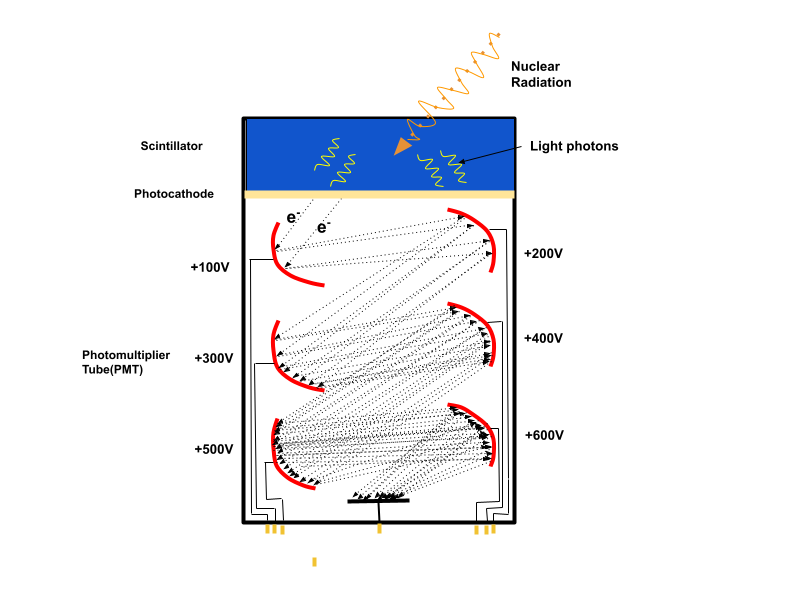
\includegraphics[width=15cm]{images/Fig2_Scintillator_detector.png}
    \caption{Scintillation Detector, showing the multiplication of electron in Photo multiplier Tube}
    \label{fig:2}
\end{figure}

\begin{multicols}{2}
\section{Development of IOSFDs}
\citeauthor{swinth1976biomedical} were the first to use IOSFD for low-background, low-energy biological photon counting, to the best of our knowledge.A huge chunk of NaI: Tl crystal was linked to a bundle of glass optical fibres in the biomedical radiation-sensitive probe. The probe was more sensitive than a diode dosimeter created for the same purpose to low-energy $^{239}Pu$ photons (17 keV, 60 keV). In addition to detecting ionising $X-/\gamma-rays$, researchers have looked at the possibility of IOSFDs for dosimetry of biological particle radiations. \citeauthor{jang2011fiber} examined the capacity of several scintillator-coupled optical fibre dosimeters to detect -rays (electrons). The sensor tip is made of Inorganic Scintillator and plastic optical fibre bundles, as illustrated in Figure 3a. To choose the optimum scintillator for a metal hydride tritium source, three types of scintillators ($Gd_2O_2S:Tb$, $Y_3Al_5O_{12}:Ce$, and $CsI:Tl$) were employed for sensor fabrication(Figure 3b). In terms of produced photons, the IOSFDs with $Gd_2O_2S:Tb$ had the best scintillation response among the three scintillators. IOSFDs with various types of scintillators and configurations have been created in recent decades, and their potential application for radiotherapy dosimetry such as external radiotherapy dosimetry, small-field in-vivo dosimetry, and BT(brachytherapy) has been examined. The re-search on IOSFDs for X-ray radiotherapy dosimetry will be covered in the next sections, as will efforts to use IOSFDs for BT dosimetry, PT, and BNCT.
\end{multicols}
\begin{figure}[H]
    \begin{subfigure}{0.5\textwidth}
    \centering
    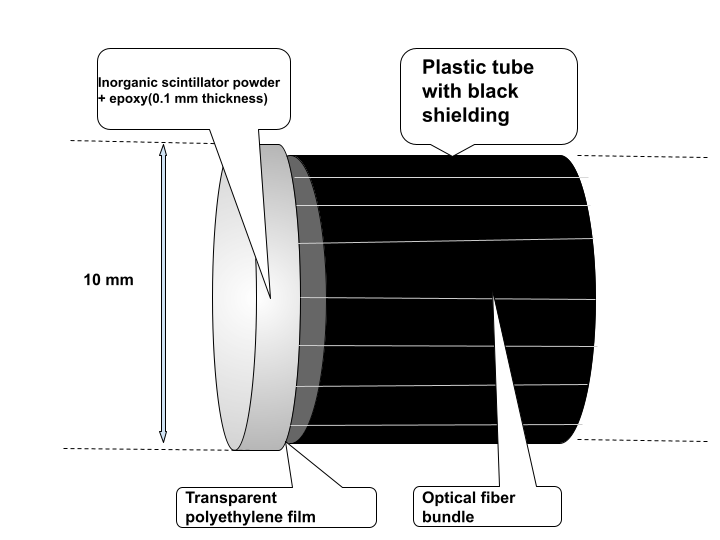
\includegraphics[width=\linewidth]{images/sensor tip.png}
    \caption{A schematic diagram of sensor tip}
    \label{fig:fig3a}
    \end{subfigure}
    \begin{subfigure}{0.5\textwidth}
    \centering
    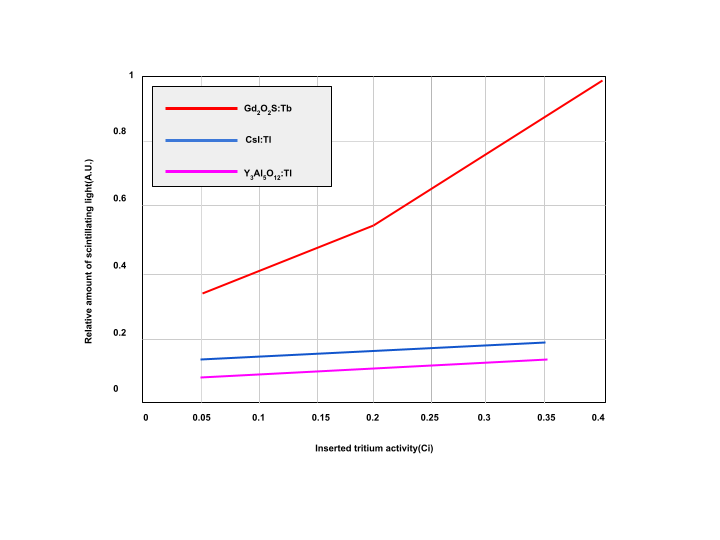
\includegraphics[width=\linewidth]{images/graph.png}
    \caption{Measured amounts of scintillation photon with three kinds of IOS}
    \label{fig:fig3b}
    \end{subfigure}
    \caption{IOSFD for detection of tritium}
\end{figure}

\begin{multicols}{2}
\section{Challenges of IOSFDs for radiotherapy dosimeter application}

Although there has been significant development in IOSFD research in recent years, there is still some worry about the clinical use of IOSFDs for in vivo dosimetry. The PDD(percentage depth dose) divergence from the normal IC(Integrated Circuit)  measurement, angle dependency, and the Cherenkov effect are three important issues in this study field that will be discussed in this section.

\subsection{PDD deviation from the standard IC measurement}
The PDD curve is used to calculate the proportion of dose deposited in water at various depths relative to the maximum dose point. In most cases, SFDs curves are compared to typical IC curves. The water-equivalent quality of the plastic organic scintillators and plastic optical fibres is one of PSFDs(plastic scintillator optical fiber dosimeters) most appealing features; as a result, PSFDs generally has no effect on dosage distribution\cite{robinson2020monte}. Early re-search on PSFDs revealed a high level of agreement with IC on the PDD test. When the detector was positioned perpendicular to the centre axis of a 10 MV X-ray radiation beam (field size 10 10 cm2), a maximum inaccuracy of 0.3 percent was reached by ignoring the Cherenkov effect. However, as compared to the IC measurement, the majority of IOSFDs showed non-ignorable deviations in depth-dose characteristics. This has remained the greatest stumbling block to IOSFD's clinical applicability to far. When the field size is bigger than 10 10 cm2 (at 1.5 cm in water equivalent material where the radiation dose reaches maximum (Dmax) for a 6-MV photon beam recorded by the IC), the $Gd_2O_2S$:Tb-based IOSFD exhibits overresponse to the X-ray (6 MV, 100 MU). As the field size grew larger, the divergence grew larger. The extent of the deviation is determined by the kind of scintillator, the incident radiation beam profile, and the sub-surface depth, among other factors.

\subsection{Angular dependence}

Angular dependency is also discussed frequently in the research on IOSFDs. The geometrical asymmetry of the scintillator material at the sensor tip causes the angular dependency. The scintillation portion is generally formed in the form of a cylinder geometry with a small diameter (less than 1 mm) and relatively long length for better coupling with the optical fibre (several millimeters). Photons or electrons entering the cylindrical sensor tip from various places and orientations may have varying beginning energy and travel further down varied length routes in the scintillator material as the angle changes. As a result, it's logical to assume that angular shifts might produce a fluctuation in radiation sensitivity. The reaction of the IOSFD to radiation with regard to angular variations along the axial and azimuthal directions of the scintillator and optical fibre has various properties when considering geometrical symmetry. As demonstrated by \citeauthor{zhuang2016embedded} and \citeauthor{alharbi2018dosimetric}, IOSFDs with cylindrical sensor tips have good axial angular independence but substantial azimuth angular dependency. From the standpoint of geometry, a solution to this problem has been proposed \cite{martinez2017characterization}. In comparison to a cylinder-shaped scintillator tip, the scintillator powders were dispersed in a quasi-sphere droplet. With an observed fluctuation of less than 2\%, the probe with this quasi-spherical shape demonstrated superior azimuth angle independence. As a result, by adjusting the shape of the scintillator material pack, angular independence may be achieved.

\subsection{Cherenkov effect in IOSFDs}

When applying SFDs for dosimetry, the Cherenkov effect is considered a substantial interference. It explains the phenomenon of electromagnetic radiation being emitted when charged particles (such as electrons and positrons) move through a medium faster than the phase velocity of light in that medium. At electron energies of around 180 keV, it may be found in practically any transparent material (e.g., silica or plastic optical fibre). The Cherenkov light signal has a broad wavelength range, extending from UV to infrared\cite{ashraf2020dosimetry}. The dosimeter's accuracy is limited by Cherenkov radiation from the optical fibre and scintillators. The Cherenkov radiation has the same strength as the plastic scintillator's scintillation signal, hence it must be eliminated if PSFD is to be used. The scintillation signal in IOSFD has a substantially higher intensity than the Cherenkov signal. Nonetheless, the Cherenkov effect must be removed and just the scintillation signal must be accounted for. 

\section{Conclusion}
This study reviewed the recent work in the field of IOSFDs, starting with some basic fundamental of SFDs, we looked at the development of IOSFDs. We have also looked at the challenges of IOSFDs and work done to resolve those issue.  Studies of embedded structures,  The use of IOSFDs and sensor tip modification proves that by adjusting the scintillator coupling technique, the coupling efficiency between the scintillator and the optical fibre may be improved. Furthermore, using a spectrum filtering approach, various IOSs with the brilliant red emission maximum make it easier to suppress the Cherenkov effect and stem effect in the optical fibre. IOSFD has the potential to be used for dosimetry in BT, PT, and BNCT, however issues such as quenching must be addressed. In the future, different IOSs' response characteristics to radiation dosage from diverse charged particle sources should be explored. 
\end{multicols}

\printbibliography

\end{document}
